\documentclass{cubeamer}
\usepackage{listings}

\title{How to \LaTeX: a (too) short introduction}
\subtitle{Journal Club}
\author[Janek Gr\"ohl]{Janek Gr\"ohl}
\date{\today} % or whatever the date you are presenting in is
\institute[University of Cambridge]{Cancer Research UK Cambridge Institute, University of Cambridge\\
Department of Physics, University of Cambridge}
% \copyrightnotice{Published by the American Institute of Aeronautics and Astronautics, Inc., with permission}

\begin{document}

\maketitle

\cutoc

\section{What is \LaTeX?}

\begin{frame}{It's pronounced "$\Lambda\alpha\theta\epsilon\chi$".}
\begin{minipage}{0.45\textwidth}
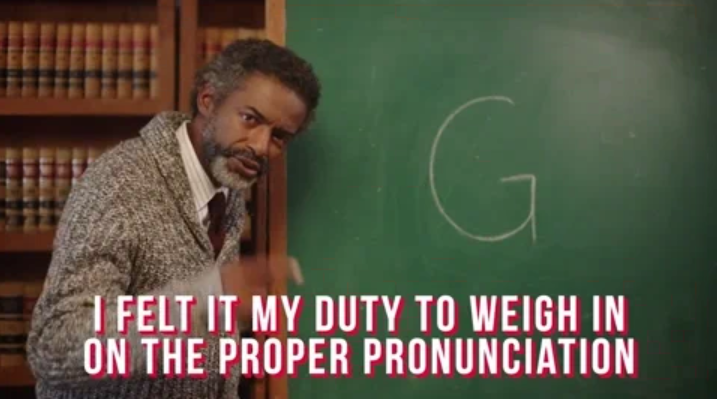
\includegraphics[width=0.9\textwidth]{img/pronunciation.png}
\end{minipage}
\begin{minipage}{0.5\textwidth}
    \textit{Insiders pronounce the χ of TeX as a Greek chi, not as an ‘x’, so that TeX rhymes with the word blecchhh. It’s the ‘ch’ sound in Scottish words like loch or German words like ach; it’s a Spanish ‘j’ and a Russian ‘kh’. \textbf{\color{red} When you say it correctly to your computer, the terminal may become slightly moist.}} \cite{knuth1984texbook}
\end{minipage}
\end{frame}

\begin{frame}{Separation of Content from Style}
\begin{minipage}{0.45\textwidth}
Content:\\
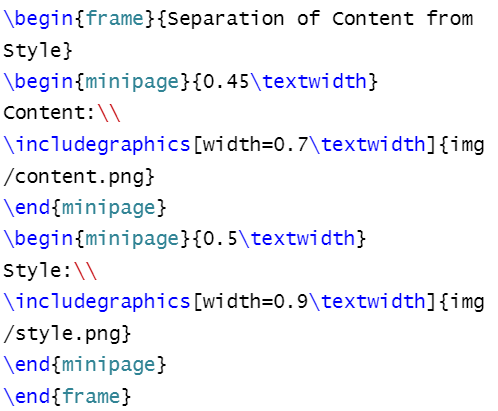
\includegraphics[width=0.7\textwidth]{img/content.png}
\end{minipage}
\begin{minipage}{0.5\textwidth}
Style:\\
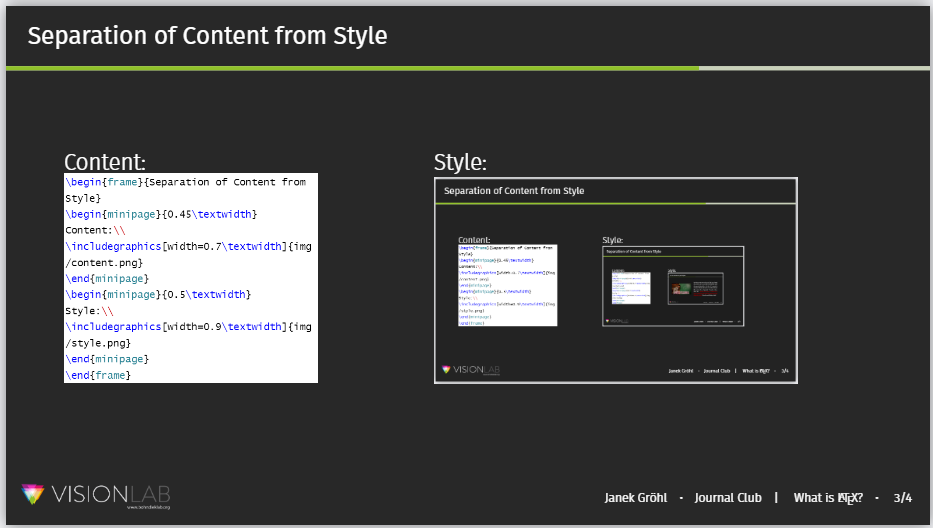
\includegraphics[width=0.9\textwidth]{img/style.png}
\end{minipage}
\end{frame}

\begin{frame}[fragile]{Minimal example for LaTeX document structure}

\begin{verbatim}
    \documentclass[12pt,a4paper]{article}
    \begin{document}
        \title{Title}   \author{Name}   \date{\today}
        
        \maketitle
        
        \section{First section}
        \subsection{Subsection}
        \section{Second section}
        
        \bibliography{bibliography_file.bib}
    \end{document}
\end{verbatim}

\end{frame}

\begin{frame}[fragile]{Document Structure Commands}
    \begin{tabular}{lll}
         \textbf{Command} &	\textbf{Level} &	\textbf{Comment}\\
         \\
         \hline
        \verb+\part{''part''}+ & -1 &not in letters\\
        \verb+\chapter{''chapter''}+ & 0 & only books and reports\\
        \verb+\section{''section''}+ &	1 &	not in letters\\
        \verb+\subsection{''subsection''}+ & 2 & not in letters\\
        \verb+\subsubsection{''subsubsection''}+ & 3 & not in letters\\
        \verb+\paragraph{''paragraph''}+ & 4 & not in letters\\
        \verb+\subparagraph{''subparagraph''}+ & 5 & not in letters\\
        \hline
    \end{tabular}
\end{frame}

\begin{frame}[fragile]{Document Structure Commands (without explicit numbering)}
    \begin{tabular}{lll}
         \textbf{Command} &	\textbf{Level} &	\textbf{Comment}\\
         \\
         \hline
        \verb+\part*{''part''}+ & -1 &not in letters\\
        \verb+\chapter*{''chapter''}+ & 0 & only books and reports\\
        \verb+\section*{''section''}+ &	1 &	not in letters\\
        \verb+\subsection*{''subsection''}+ & 2 & not in letters\\
        \verb+\subsubsection*{''subsubsection''}+ & 3 & not in letters\\
        \verb+\paragraph*{''paragraph''}+ & 4 & not in letters\\
        \verb+\subparagraph*{''subparagraph''}+ & 5 & not in letters\\
        \hline
    \end{tabular}
\end{frame}

\section{Why use \LaTeX?}

\begin{frame}{Situations where I used \LaTeX \space in the past}
\begin{itemize}
    \item Creating a book for my Analysis I \& II tutoring students
    \item My bachelors thesis
    \item My masters thesis
    \item My PhD thesis
    \item Any (internal) literature reviews
    \item All of my papers (I think)
\end{itemize}
\end{frame}

\subsection{Large documents}

\begin{frame}{Word and other WYSIWYG editors seem to struggle with large files..}
\begin{itemize}
    \item Lagging and slow behaviour when scrolling and editing
    \item Errors in PDF exporting
    \item Rendering errors for figures
    \item Formatting issues arising somewhere in the document when editing somewhere else
    \item Corruption of files when saving / opening
\end{itemize}
\end{frame}

\begin{frame}{Why is \LaTeX\space any better?}
\begin{itemize}
    \item The content is editable independently of the formatting
    \item Very small computational requirements during editing
    \item Possibility to easily sub-divide chapter into different files
    \item Even year-old documents (both the PDFs and the \LaTeX\space files) are readable
    \item Not reliant on the "mood" of any particular vendor
\end{itemize}
\end{frame}

\subsection{Math notation}

\begin{frame}{Math notation with \LaTeX}
    \begin{itemize}
        \item Super powerful script-based notation
        \item Started by enclosing a statement in dollar signs (\$ MATH \$)
        \item Pre-defined Greek and Hebrew letters ($\alpha, \beta, \gamma, ...$)
        \item Math constructs (fractions, integrals, sums, ...)
        \item Delimiter symbols, standard function names, operator symbols, ...
    \end{itemize}
\end{frame}

\begin{frame}[fragile]{Some examples}
    \begin{tabular}{cc}
    TeX command & Rendering \\
    \hline
    \\
      \tiny{\verb!\int\limits_0^\infty\dfrac{e^x}{1+2e^x+e^{2x}}dx!}   & $ \int\limits_0^\infty \dfrac{e^x}{1+2e^x+e^{2x}} dx$  \\
    \\
    \tiny{\verb!\sum\limits_{-\infty}^{\infty} \dfrac{1}{2} a_k - ib_k)!} & 
    $ \sum\limits_{-\infty}^{\infty} \dfrac{1}{2} (a_k - ib_k) $ \\
    \\
    \tiny{\verb!f(x_1, y_1)=\left(\begin{matrix} x_1\\ y_1 \end{matrix}\right)!} &
    $f(x_1, y_1)=\left(\begin{matrix} x_1\\ y_1 \end{matrix}\right)$\\
    \end{tabular}
\end{frame}

\subsection{Bibliography management}

\begin{frame}{BibTeX}
    \begin{itemize}
        \item BibTeX is a tool and a file format used to describe and process references
        \item References are kept in a .bib file
        \item References can then be used throughout a \LaTeX\space document
        \item Complete control of the way references are used in the text and how the bibliography is formatted
    \end{itemize}
\end{frame}

\begin{frame}{.bib File content example}
\hspace{0.2\textwidth}
\begin{minipage}{0.6\textwidth}
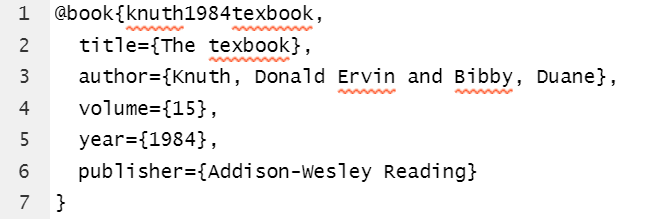
\includegraphics[width=\textwidth]{img/bib file content.png}
\end{minipage}
\end{frame}

\begin{frame}{Citing in the text}

\begin{itemize}
    \item \textbackslash cite\{knuth1984texbook\} \cite{knuth1984texbook}
    \item \textbackslash cite[p.42]\{knuth1984texbook\} \cite[p.42]{knuth1984texbook}
\end{itemize}
    
\end{frame}

\section{What are the problems with \LaTeX?}

\begin{frame}{The one \LaTeX to rule them all?}
\hspace{0.25\textwidth}
\begin{minipage}{0.5\textwidth}

\includegraphics[width=\textwidth]{img/meme.jpg}
\end{minipage}
    
\end{frame}

\begin{frame}{Drawbacks}
    \begin{itemize}
        \item Learning Curve
        \item Counterintuitivity
        \item Setting it up on a local computer
    \end{itemize}
\end{frame}

\section{A practical guide to \LaTeX (live demo)}

\begin{frame}{Useful links and resources}
    \begin{itemize}
        \item Code to this presentation:
        \url{https://github.com/jgroehl/HowToLaTeX}
        \item Overleaf: \url{https://www.overleaf.com/}
        \item CamTeX society: \url{https://camtex.soc.srcf.net/}
        \item LyX: \url{https://www.lyx.org/}
        \item Google Scholar Button: \url{https://chrome.google.com/webstore/detail/google-scholar-button/ldipcbpaocekfooobnbcddclnhejkcpn?hl=en}
    \end{itemize}
\end{frame}

\begin{frame}{Bibliography}
\bibliographystyle{apalike}
\bibliography{bibliography.bib}
\end{frame}

\end{document}
